\section{Sketch}
\label{sec:sketch}

MARK: \blue{Blue is used for hint and comments.} \red{Red is used for issues, problems.}

\begin{itemize}[\blue{Storyline:} $\leftarrow$ we keep the sketch of the storyline currently here only to have a overall view for the draft. This part will be deleted later on]
    \item \begin{itemize}[Introduction]
        \item 3-4 paragraphs (Broad topic, problem, solution and contributions)
        \item   \begin{itemize}[Motivation]
            \item Latency is critical in the next generation of communication networks (e.g. for Tactile Internet)
            \item \blue{To be solved Problem} How to implement low latency VNFs in \blue{Virtual Machine}(Containers are
                not considered in this work)?
                \begin{enumerate}
                    \item In kernel space or in user space? Pros and cons?
                    \item Which frameworks should be used? Pros and Cons should be analyzed in a separate section.
                    \item How to enable low latency without decreasing other features and performance parameters too
                        much? e.g. Flexibility, Scalability for multiple VNFs. Bandwidth, hardware resource usage(related to
                        energy consumption). \blue{The chain-based approach proposed in this paper can better meet these requirements.}
                \end{enumerate}
        \end{itemize}
\end{itemize}

\item \begin{itemize}[Related Work]

    \item \begin{itemize}[Packet IO frameworks related papers]
        \item User space: High performance Packet IO
        \item Kernel space: XDP and eBPF in practice(2 papers are found).
    \end{itemize}

\item \begin{itemize}[Virtualed Network Functions Approaches]
    \item Vitualized Network Coding on the Internet. \blue{This paper implement NC with DPDK KNI for flexibility}.
    \item \todo{Find other approaches to achieve low latency VNFs}
\end{itemize}

\end{itemize}

\item \begin{itemize}[Low latency VNF]
    \item Compare different frameworks and explain why XDP and DPDK are finally chosen for further implementation.
    \item Compare chain-based approach and KNI-based approach. \blue{Describe OVS-DPDK is the tech which reduce the
            latency overhead introduced by the chain-based approach, the context switching between user- and kernel space is
        the main issue that increase the latency with KNI approach}

        \begin{figure}[htpb]
            \centering
            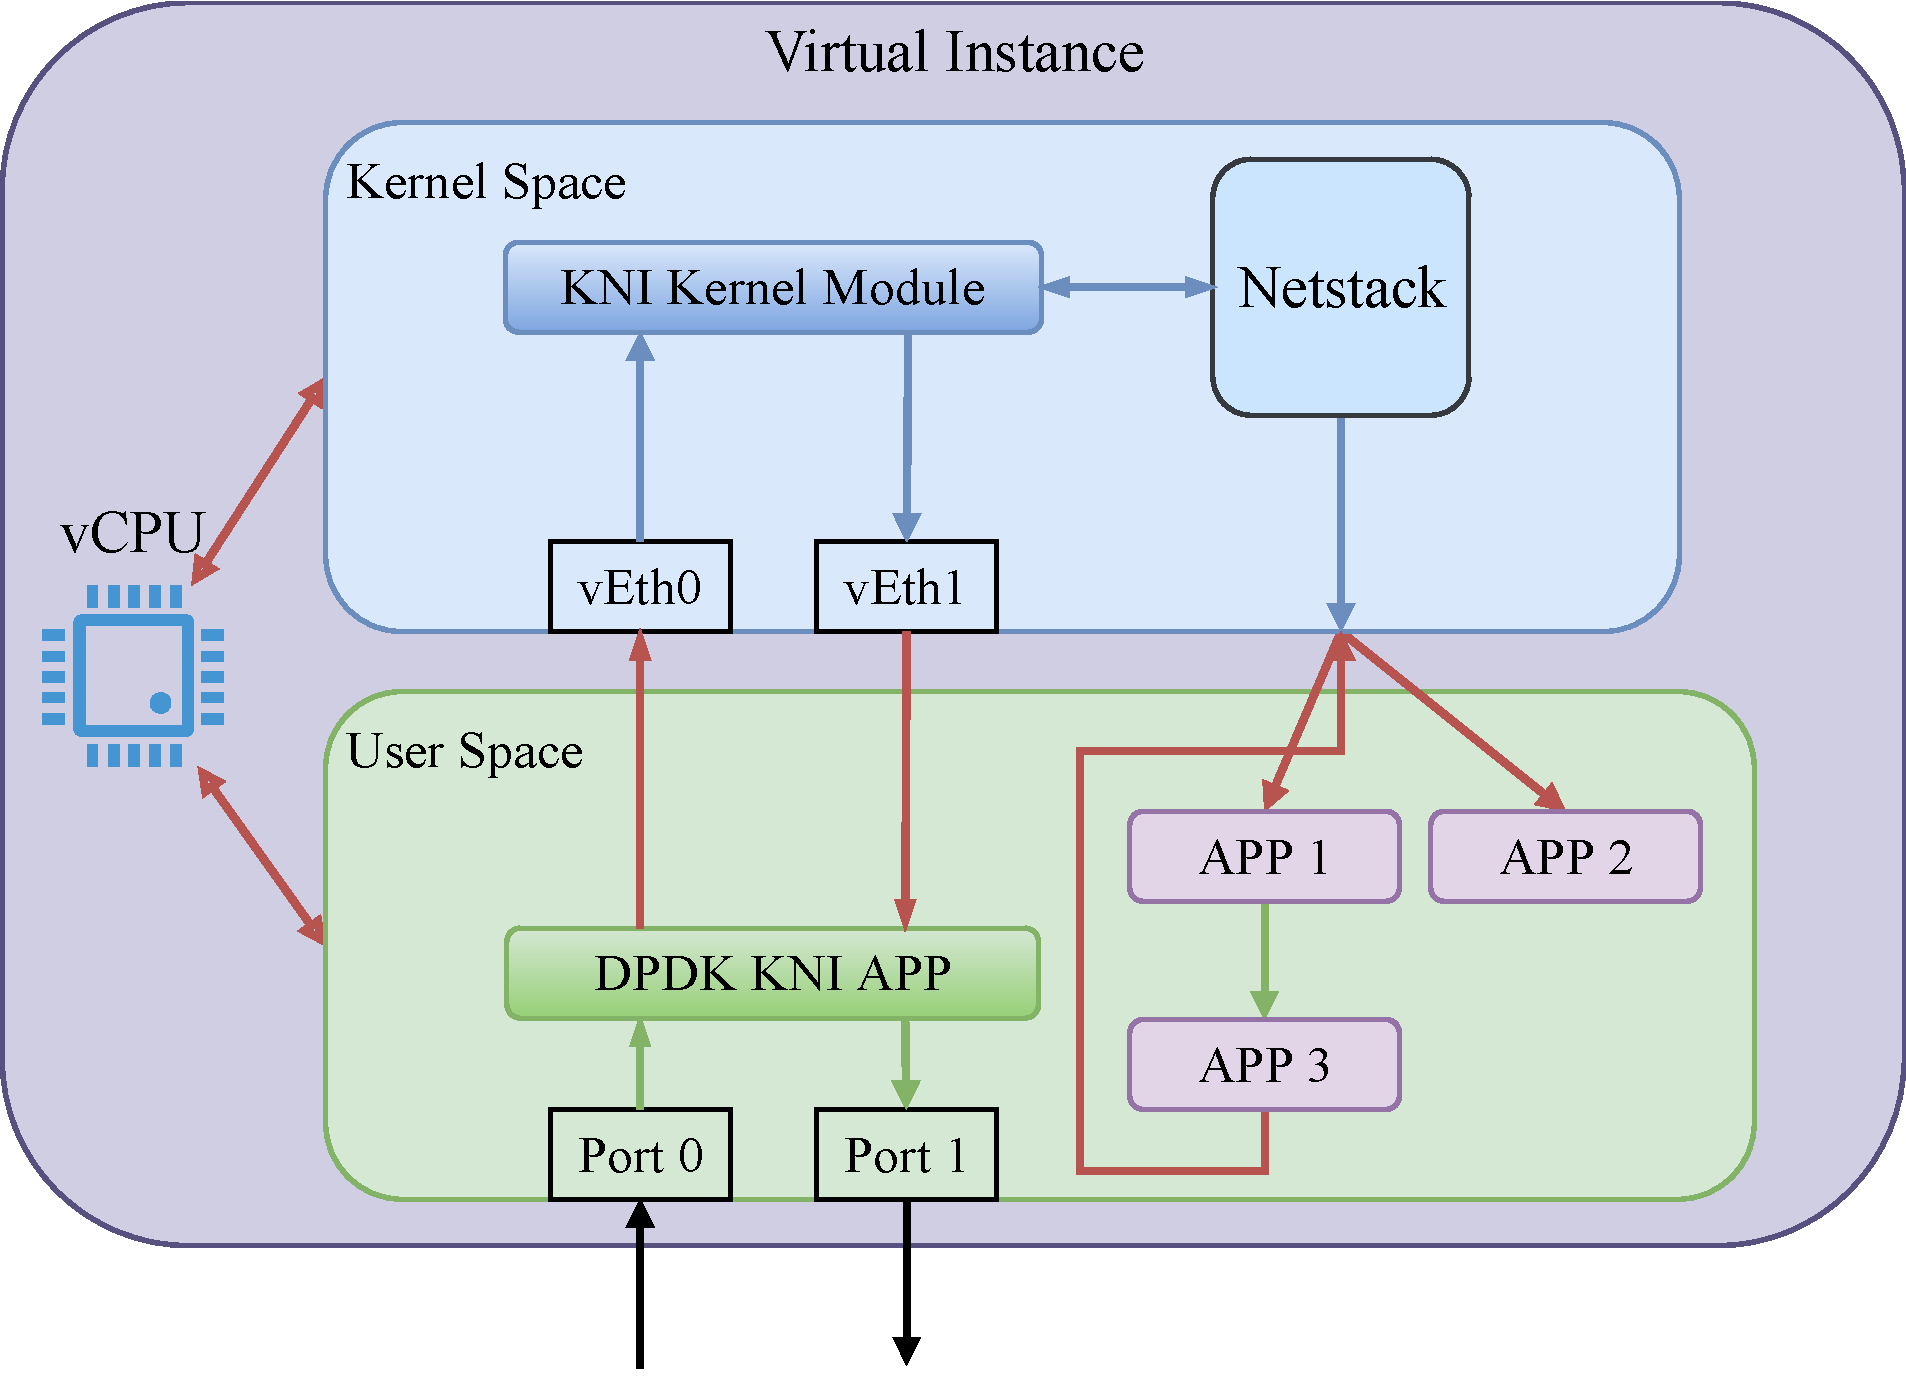
\includegraphics[width=0.8\linewidth]{./figures/KNI_Approach.pdf}
            \caption{KNI Approach}
            \label{fig:kni_approach}
        \end{figure}

        \begin{figure}[htpb]
            \centering
            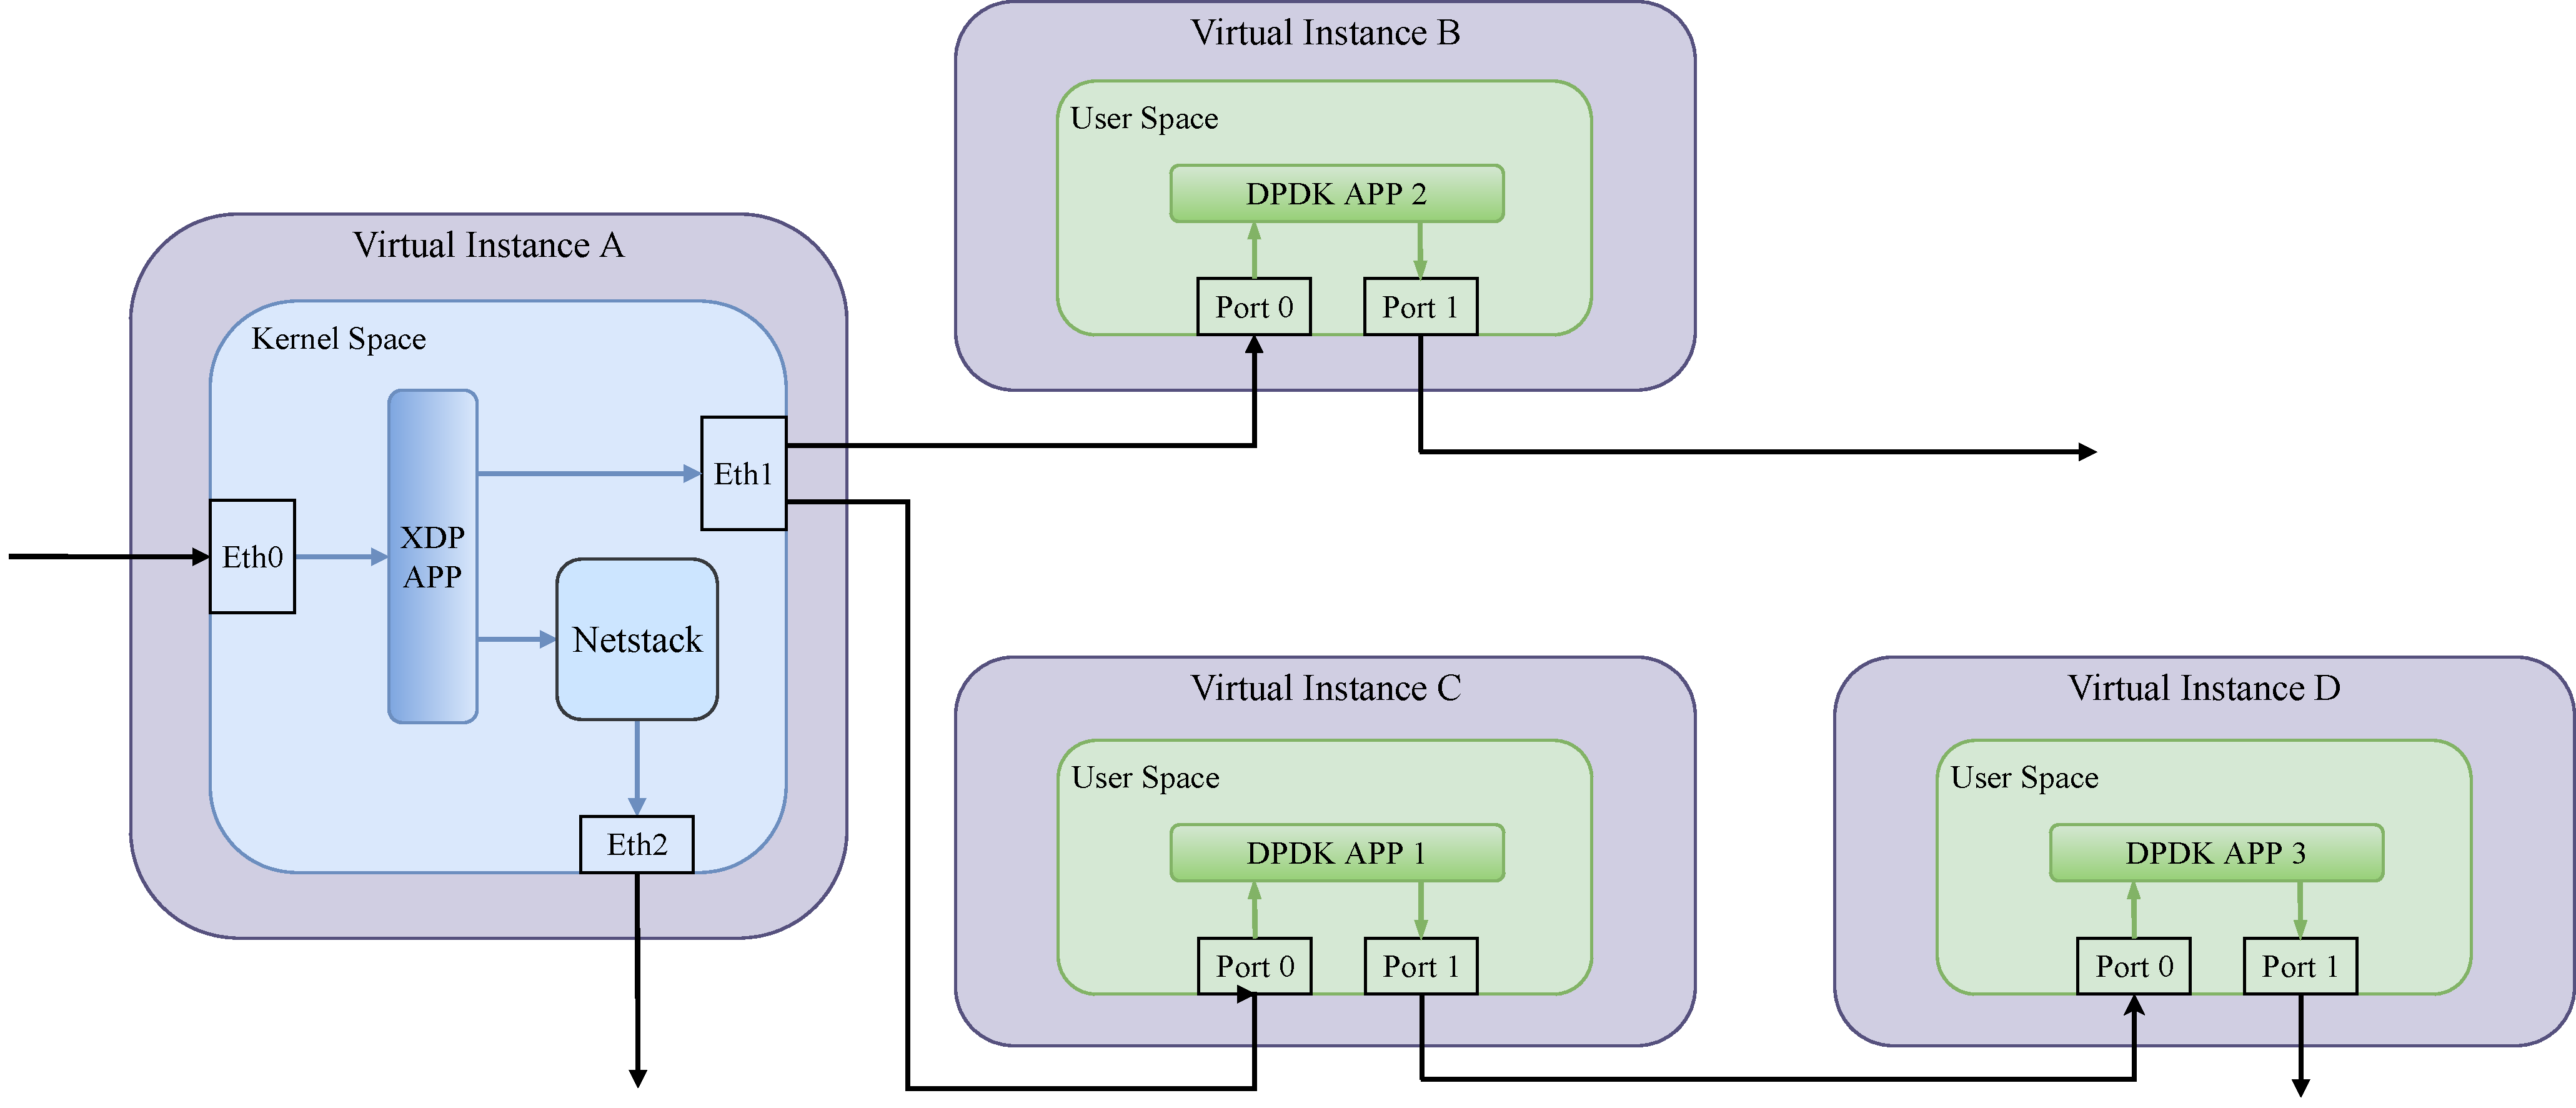
\includegraphics[width=0.8\linewidth]{./figures/Chain_Approach.pdf}
            \caption{Chain Approach}
            \label{fig:chain_approach}
        \end{figure}


    \item Describe how to enable our approach on the OpenStack cloud platform. \blue{Use SFC, enable multi-queue feature
        of the Nova.}
\end{itemize}


\item \begin{itemize}[Measurement Results]
    \item End-to-End latency of KNI and XDP+DPDK (1. 1 core for all; 2 cores to make them fair)
    \item Bandwidth of KNI and XDP+DPDK. (Different burst size can be a variable here.)
    \item CPU usage of KNI and XDP+DPDK on the physical node. \blue{Nova compute node}
\end{itemize}

\begin{table}[htbp]
    \begin{tabular}{|c|c|c|c|c|c|}
        \hline
        Approach        & User & System & IO-Wait & Guest & Total \\ \hline
        DPDK KNI 1 vCPU & 25.21 & 23.35  & 0.04    & 1.70  & 50.3  \\ \hline
        DPDK KNI 2 vCPU & 25.23 & 47.18  & 0.04    & 2.88  & 75.33 \\ \hline
        XDP + DPDK      & 25.24 & 22.97  & 0.04    & 2.18  & 50.43 \\ \hline
    \end{tabular}
    \caption{CPU usage of the compute node (in percent)}
\end{table}

\item \begin{itemize}[Conclusion]
    \item If latency counts, our approach is better.
\end{itemize}

\item \begin{itemize}[Future Work]
    \item Extend SFC-extension to support fully chain-based approach on OpenStack.
\end{itemize}



    \end{itemize}
